\documentclass{article}
\usepackage{cmap}
\usepackage[utf8]{inputenc}
\usepackage[english,ukrainian]{babel}
\usepackage{graphicx}
\usepackage{geometry}
\usepackage{listings}
\usepackage{float}
\usepackage{multicol}
\geometry{
	a4paper,
	left=20mm,
	right=20mm,
	top=20mm,
	bottom=20mm
}
\lstset{
	language=c,
	tabsize=4,
	keepspaces,
	showstringspaces=false,
}
\graphicspath{ {./pictures} }
\setlength{\parindent}{4em}

\newcommand\subject{Алгоритми та структури даних}
\newcommand\lecturer{доцент кафедри ПЗ\\Коротєєва Т.О.}
\newcommand\teacher{асистент кафедри ПЗ\\Франко А.В.}
\newcommand\mygroup{ПЗ-22}
\newcommand\lab{9}
\newcommand\theme{НЕЛІНІЙНІ СТРУКТУРИ ДАНИХ: ЧЕРВОНО-ЧОРНІ ДЕРЕВА }
\newcommand\purpose{ознайомитися з червоно-чорними деревами та отримати навички програмування алгоритмів, що їх обробляють. }

\begin{document}
	\begin{normalsize}
		\begin{titlepage}
			\thispagestyle{empty}
			\begin{center}
				\textbf{МІНІСТЕРСТВО ОСВІТИ І НАУКИ УКРАЇНИ\\
					НАЦІОНАЛЬНИЙ УНІВЕРСИТЕТ "ЛЬВІВСЬКА ПОЛІТЕХНІКА"}
			\end{center}
			\begin{flushright}
				Інститут \textbf{КНІТ}\\
				Кафедра \textbf{ПЗ}
			\end{flushright}
			\vspace{200pt}
			\begin{center}
				\textbf{ЗВІТ}\\
				\vspace{10pt}
				До лабораторної роботи № \lab\\
				\textbf{На тему}: “\textit{\theme}”\\
				\textbf{З дисципліни}: “\subject”
			\end{center}
			\vspace{112pt}
			\begin{flushright}
				
				\textbf{Лектор}:\\
				\lecturer\\
				\vspace{28pt}
				\textbf{Виконав}:\\
				
				студент групи \mygroup\\
				Коваленко Д.М.\\
				\vspace{28pt}
				\textbf{Прийняв}:\\
				
				\teacher\\
				
				\vspace{28pt}
				«\rule{1cm}{0.15mm}» \rule{1.5cm}{0.15mm} 2022 р.\\
				$\sum$ = \rule{1cm}{0.15mm}……………\\
				
			\end{flushright}
			\vspace{\fill}
			\begin{center}
				\textbf{Львів — 2022}
			\end{center}
		\end{titlepage}
		
		\begin{description}
			\item[Тема.] \theme.
			\item[Мета.] \purpose.
		\end{description}
		
		\section*{Лабораторне завдання}

	Розробити програму, яка:
		\begin{center}
			\begin{enumerate}
				\item читає з клавіатури ключі N, M (цілі, дійсні або символи залежно від варіанту завдання);
				\item програма зберігає першу послідовність до червоно-чорного дерева;
				\item кожного разу, коли до дерева додається новий елемент, потрібно вивести статистику (згідно з варіантом завдання);
				\item після побудови дерева для кожного елемента другої послідовності М потрібно вивести результати наступних операцій над деревом: 
				\item 1. Чи є елемент у дереві та його колір?
				
				2. Нащадок (нащадки) та його (їх) колір.
				
				3. Батько та його колір. 
			\end{enumerate}
		Варіант 2: N, M – дійсні; мінімальний елемент та його колір; батько та його колір. 
		\end{center}
		
		\section*{Теоретичні відомості}
		Дерева як засіб реалізації словників ефективні, якщо їх висота мала, але мала висота не гарантується, і в гіршому випадку дерева не більш ефективні, ніж списки. Червоно-чорні дерева – це один з типів збалансованих дерев пошуку, в яких передбачені операції балансування гарантують, що висота дерева не перевищить O(log N).
		
		Червоно-чорне дерево (red-black tree) – це двійкове дерево пошуку, вершини якого розділені на червоні (red) і чорні (black). Таким чином, кожна вершина зберігає один додатковий біт – її колір.
		
		При цьому повинні виконуватися певні вимоги, які гарантують, що глибина будь-яких двох листків дерева відрізняється не більше, ніж у два рази, тому дерево можна назвати збалансованим (balanced).
		
		Кожна вершина червоно-чорного дерева має поля color (колір), key (ключ), left (лівий нащадок), right (правий нащадок) і p (предок). Якщо у вершини відсутній нащадок або предок, відповідне поле містить значення nil. Для зручності ми будемо вважати, що значення nil, які зберігаються в полях left і right, є посиланнями на додаткові (фіктивні) листки дерева. При такому заповненні дерева кожна вершина, що містить ключ, має двох нащадків.
		
		Двійкове дерево пошуку називається червоно-чорним деревом, якщо воно має такі властивості (будемо називати їх RB-властивостями, red-black properties): 
		
		\section*{Хід роботи}
		\begin{lstlisting}[language=C]
mod rbtree;

use rbtree::RBTree;

use eframe::egui::{
	self,
	text_edit::TextEdit,
};
use egui_extras::{Size, TableBuilder};

fn main() {
	let options = eframe::NativeOptions::default();
	eframe::run_native(
	"Stack",
	options,
	Box::new(|_cc| Box::new(App::default())),
	);
}

struct App {
	n: String,
	m: String,
	min: Option<usize>,
	v_to_find: String,
	found_key: Option<usize>,
	ntree: RBTree<usize, f32>,
	mtree: RBTree<usize, f32>,
}

impl Default for App {
	fn default() -> Self {
		Self {
			n: String::new(),
			m: String::new(),
			min: None,
			v_to_find: String::new(),
			found_key: None,
			ntree: RBTree::new(),
			mtree: RBTree::new(),
		}
	}
}

impl eframe::App for App {
	fn update(&mut self, ctx: &egui::Context, _frame: &mut eframe::Frame) {
		egui::CentralPanel::default().show(ctx, |ui| {
			ui.heading("Red Black Tree");
			ui.horizontal(|ui| {
				if ui.button("Add").clicked() {
					if let Ok(v) = self.n.parse::<f32>() {
						if let Some(l) = self.ntree.get_last() {
							self.ntree.insert(l.0 + 1, v);
						} else {
							self.ntree.insert(0, v);
						}
					}
					let mut min = f32::MAX;
					for (&k, &v) in self.ntree.iter() {
						if v < min {
							min = v;
							self.min = Some(k);
						}
					}
				}
				ui.add(TextEdit::singleline(&mut self.n)
				.hint_text("N")
				.desired_width(100.0)
				);
			});
			ui.horizontal(|ui| {
				if let Some(min) = self.min {
					ui.label(format!("Min: {}", self.ntree.get(&min).unwrap()));
					ui.label(format!("Min Color: {:?}", self.ntree.color(min)));
					if let Some(parent) = self.ntree.parent(min) {
						ui.label(format!("Min Parent: {}", self.ntree.get(&parent).unwrap()));
						ui.label(format!("Min Parent Color: {:?}", self.ntree.color(parent)));
					}
				}
			});
			ui.horizontal(|ui| {
				if ui.button("Add").clicked() {
					if let Ok(v) = self.m.parse::<f32>() {
						if let Some(l) = self.mtree.get_last() {
							self.mtree.insert(l.0 + 1, v);
						} else {
							self.mtree.insert(0, v);
						}
					}
				}
				ui.add(TextEdit::singleline(&mut self.m)
				.hint_text("M")
				.desired_width(100.0)
				);
			});
			ui.horizontal(|ui| {
				if ui.button("Find").clicked() {
					if let Ok(v_to_find) = self.v_to_find.parse::<f32>() {
						for (&k, &v) in self.mtree.iter() {
							if v == v_to_find {
								self.found_key = Some(k);
								break;
							}
						}
					}
				}
				ui.add(TextEdit::singleline(&mut self.v_to_find)
				.hint_text("Find")
				.desired_width(100.0)
				);
				ui.label(format!("Found: {}", self.found_key.is_some()));
			});
			if let Some(found) = self.found_key {
				if let Some(left) = self.mtree.left(found) {
					ui.horizontal(|ui| {
						ui.label(format!("Left: {}", self.mtree.get(&left).unwrap()));
						ui.label(format!("Color: {:?}", self.mtree.color(left)));
					});
				}
				if let Some(right) = self.mtree.right(found) {
					ui.horizontal(|ui| {
						ui.label(format!("Right: {}", self.mtree.get(&right).unwrap()));
						ui.label(format!("Color: {:?}", self.mtree.color(right)));
					});
				}
				if let Some(parent) = self.mtree.parent(found) {
					ui.horizontal(|ui| {
						ui.label(format!("Parent: {}", self.mtree.get(&parent).unwrap()));
						ui.label(format!("Color: {:?}", self.mtree.color(parent)));
					});
				}
			}
		});
	}
}

		\end{lstlisting}
		
		\begin{figure}[H]
			\centering
			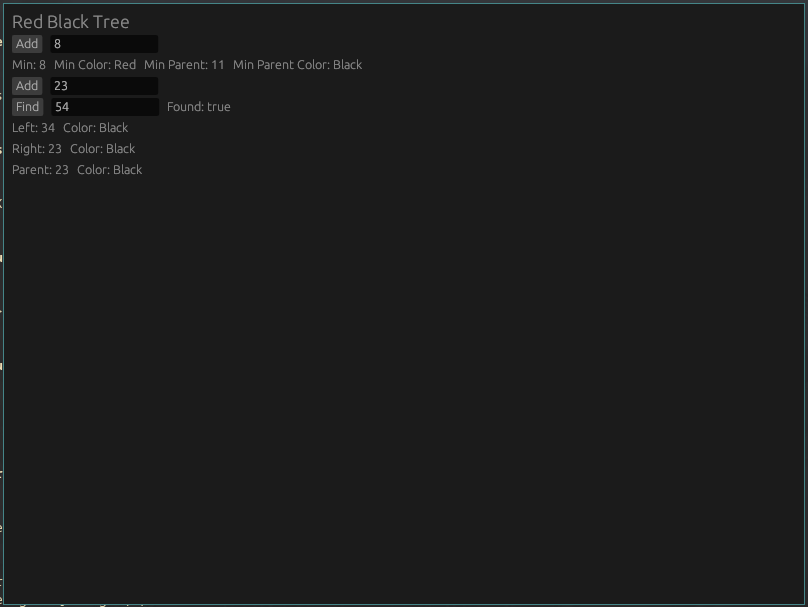
\includegraphics[scale=0.6]{1}	
			\caption{Виконання програми}
		\end{figure}
	
	\begin{figure}[H]
		\centering
		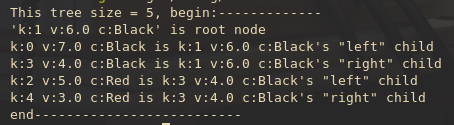
\includegraphics[scale=0.8]{2}	
		\caption{Вивід червоно чорного дерева}
	\end{figure}
		
		\section*{Висновоки}
		Під час виконання лабораторної роботи я ознайомився з червоно-чорними деревами та отримав навички програмування алгоритмів, що їх обробляють. 
		
	\end{normalsize}
\end{document}
